\section{\label{sec:results}Primary Results}


% \subsection{\label{subsec:res_sel}Selected Results from Individual Detectors}
% Here we discuss a selection of results from individual detector experiments.
% These were chosen to highlight specific features either of the detectors themselves or of our analytical process.
% The full collection of results plots can be found in~\ref{}. %Appendix~B~\{\ref{ch:all_results}\}. 
% ~
% % c1
% % maybe NuLat-5?
% \begin{figure}[ht]
%   \begin{center}
%     % \includegraphics[width=1.0\linewidth]{figures/COMPMAIN_NULAT5_10K_bursts.png}
%     \includegraphics[width=1.0\linewidth]{figures/COMPMAIN_NULAT5_10K_bursts.png}
%     \caption{Scintillation Bursts in NuLat~$5^3$}
%     \label{fig:ind_c1}
%   \end{center}
% \end{figure}
% ~
% % c2
% % either chooz, nl5, or both
% % \begin{figure}[ht]
% \begin{sidewaysfigure}[ht]
%   \begin{center}
%     % \includegraphics[width=1.0\linewidth]{figures/COMPMAIN_CHOOZ_10k_nu-trg.png}
%     \includegraphics[width=0.9\linewidth]{figures/COMPMAIN_CHOOZ_10k_nu-trg.png}
%     \caption{Neutrino-Trigger Results in DC}
%     \label{fig:ind_c2}
%   \end{center}
% % \end{figure}
% \end{sidewaysfigure}
% ~
% % c3
% % def nl3, maybe also ch & santa
% \begin{figure}[ht]
%   \begin{center}
%     % \includegraphics[width=0.65\linewidth]{figures/COMPMAIN_NULAT_10K_pd-xyz.png}
%     \includegraphics[width=0.65\linewidth]{figures/COMPMAIN_NULAT_10K_pd-xyz.png}
%     \caption[Prompt \& Delayed Event Locations in NuLat~$3^3$]{Prompt \& Delayed Event Locations in NuLat~$3^3$ \\
%       \emph{Note: Difference in marker sizes exaggerated for visual clarity}}
%     \label{fig:ind_c3}
%   \end{center}
% \end{figure}
% ~
% % c3_with-geo
% % same?
% \begin{figure}[ht]
%   \begin{center}
%     % \includegraphics[width=0.65\linewidth]{figures/COMPMAIN/c3_with-geo/COMPMAIN_NULAT_10K_pd-xyz-with-geo.png}
%     \includegraphics[width=0.65\linewidth]{figures/COMPMAIN_NULAT_10K_pd-xyz-with-geo.png}
%     \caption[Geometry Overlay Added to Prompt \& Delayed Event Locations in NuLat~$3^3$]{Geometry Overlay Added to Prompt \& Delayed Event Locations in NuLat~$3^3$ \\
%       \emph{Note: Difference in marker sizes exaggerated for visual clarity}}
%     \label{fig:ind_c3_with_geo}
%   \end{center}
% \end{figure}
% ~
% % c4
% % def. somebody 3D
% \begin{figure}[ht]
%   \begin{center}
%     % \includegraphics[width=0.7\linewidth]{figures/COMPMAIN_NULAT5_10K_results-ang-separate.png}
%     \includegraphics[width=0.7\linewidth]{figures/COMPMAIN_NULAT5_10K_results-ang-separate.png}
%     \caption{Reconstructed Azimuthal and Polar Angles for NuLat~$5^3$}
%     \label{fig:ind_c4}
%   \end{center}
% \end{figure}
% ~
% % c5
% % BIG ONE HERE
% \begin{figure}[ht]
%   \begin{center}
%     % \includegraphics[width=0.7\linewidth]{figures/COMPMAIN_NULAT5_10K_results-cos-psi.png}
%     \includegraphics[width=0.7\linewidth]{figures/COMPMAIN_NULAT5_10K_results-cos-psi.png}
%     \caption{Cos$(\psi)$\ Distribution for NuLat~$5^3$}
%     \label{fig:ind_c5}
%   \end{center}
% \end{figure}
% ~
% % c6
% % maybe chooz, one NL, SANTA?
% \begin{sidewaysfigure}[ht]
%   \begin{center}
%     % \includegraphics[width=0.8\linewidth]{figures/COMPMAIN_NULAT5_10K_results-skymap.png}
%     \includegraphics[width=0.8\linewidth]{figures/COMPMAIN_NULAT5_10K_results-skymap.png}
%     \caption{Neutrino-Source Skymap for NuLat~$5^3$}
%     \label{fig:ind_c6}
%   \end{center}
% \end{sidewaysfigure}
% ~
% % selected results text
% \paragraph{Scintillation Bursts}
% Fig.~\ref{fig:ind_c1} shows a set of test metrics which we primarily used to ensure that our simulations were properly configured and calibrated; it is from the NuLat~$5^3$ dataset.
% Features of note include the $\nucl{6}{Li}$-capture peaks in the energy plots and their downward shifts after quenching is applied.
% \paragraph{Neutrino-Trigger Results}
% Fig.~\ref{fig:ind_c2} shows the \ibd-candidate events registered by the neutrino trigger from the \dc/monolithic dataset.
% We are particularly proud of this visualization, as we do not believe the three primary \ibd\ neutrino-trigger parameters \dash prompt energy, delayed energy, and interevent time \dash have been presented elsewhere in a single, easily-readable plot such as this.
% Features of note include the \ep\ $KE$ (and, by proxy, the approximate \nb\ $KE$) projected in red across the back and the prominent neutron-capture peaks in blue ($\nucl{1}{H}$ just above 2~MeV, and the two Gd isotopes between 7~and~8~MeV).
% \paragraph{Prompt and Delayed Event Positions}
% Fig.~\ref{fig:ind_c3} is from the NuLat~$3^3$ dataset and shows the measured positions of the prompt and delayed events.
% Note that, for visual clarity, the marker sizes for each XYZ bin are proportional not to the absolute number of entries but rather to the number of entries exceeding the minimum.
% Easily the most notable feature here is the asymmetry in the delayed-event positions, which have a clear trend increasing along the direction of \nb\ travel ($-\hat{x}$).
% \paragraph{Prompt \& Delayed Positions with Geometry Overlay}
% Fig.~\ref{fig:ind_c3_with_geo} is identical to Fig.~\ref{fig:ind_c3}, except that it features the detector geometry (again, NuLat~$3^3$ in this case) overlaid on the plot for visual reference.
% \paragraph{Reconstructed Angles to Antineutrino Source}
% Fig.~\ref{fig:ind_c4} shows the reconstructed azimuthal and polar angles from the NuLat~$5^3$ dataset.
% The quantization of the cubical lattice is quite clear in both plots.
% The true direction to the \nb\ source is $(\varphi, \theta) = (0^\circ, 90^\circ)$.
% \paragraph{$\bm{\mathrm{Cos}(\psi)}$ Distribution}
% Fig.~\ref{fig:ind_c5} shows the $\mathrm{Cos}(\psi)$ distribution from the NuLat~$5^3$ dataset.
% The quantization is again quite apparent, as is the clear trend in the forward direction (see \S\ref{sec:dirn_meth} above for interpretation of this distribution and \S\ref{subsec:ncomp_sum} below for the full collection of these plots).
% \paragraph{Skymap}
% Fig.~\ref{fig:ind_c6} shows the reconstructed azimuthal and polar angles from the NuLat~$5^3$ dataset visualized as a ``skymap'' \dash a spherical heatmap projected onto a 2D plot.\footnote{The map transformation used here is the Aitoff projection.}
% The upstream cube, representing the correct direction to the \nb\ source at $(\mathrm{lat, long}) = (0^\circ, 0^\circ)$, is visible as the primary peak in the center of the plot.
% The directions to the other neighboring cubes are likewise visible as the remaining peaks at even angular spacing around it.


\subsection{\label{subsec:res_agg}Aggregate Results}

% all cos[psi] distributions -- 2D
\begin{figure*}[ht]
  \centering
  \begin{overpic}[width=0.48\linewidth,percent]{figures/cos_psi_all_2d.png}
    \put(05.0,-02.0){\textbf{\textit{(a)} Absolute}}
    %\label{subfig:cos_psi_2d_all}
  \end{overpic}
  \unskip\ \vrule\ 
  \begin{overpic}[width=0.48\linewidth,percent]{figures/cos_psi_all_norm_2d.png}
    \put(05.0,-02.0){\textbf{\textit{(b)} Normalized}}
    %\label{subfig:cos_psi_2d_all_normalized}
  \end{overpic}
  \caption[\textbf{Summary Plot of Normalized Cos$\bm{(\psi)}$ Distributions\\for 2D Experiments}]{\textbf{Summary Plot of Normalized Cos$\bm{(\psi)}$ Distributions\\for 2D Experiments}\\The quantity $\langle \cos(\psi) \rangle$ for each experiment is given in the legend and marked on the horizontal axis.}
  \label{fig:cospsi_2d}
\end{figure*}

% all cos[psi] distributions -- 3D
\begin{figure*}[ht]
  \centering
  \begin{overpic}[width=0.48\linewidth,percent]{figures/cos_psi_all_3d.png}
    \put(05.0,-02.0){\textbf{\textit{(a)} Absolute}}
    %\label{subfig:cos_psi_3d_all}
  \end{overpic}
  \unskip\ \vrule\ 
  \begin{overpic}[width=0.48\linewidth,percent]{figures/cos_psi_all_norm_3d.png}
    \put(05.0,-02.0){\textbf{\textit{(b)} Normalized}}
    %\label{subfig:cos_psi_3d_all_normalized}
  \end{overpic}
  %\caption[\textbf{Summary Plot of Normalized Cos$\bm{(\psi)}$ Distributions\\for 3D Experiments}]{\textbf{Summary Plot of Normalized Cos$\bm{(\psi)}$ Distributions\\for 3D Experiments}\\The quantity $\langle \cos(\psi) \rangle$ for each experiment is given in the legend.}
  \caption[\textbf{Summary Plot of Cos$\bm{(\psi)}$ Distributions for 3D Experiments}]{\textbf{Summary Plot of Cos$\bm{(\psi)}$ Distributions for 3D Experiments}\\The quantity $\langle \cos(\psi) \rangle$ for each experiment is given in the legend and marked on the horizontal axis.\\``LN3 LIMIT'' indicates the simulated directional performance of a 1.5\%-wt.~$^{6}$\textbf{L}ithium-loaded, \textbf{N}on-SANTA, \textbf{3}D-reconstructing (LN3) monolithic detector with a hypothetical \emph{perfect} position resolution (\textit{i.e.,} $\delta \{x,y,z\} \equiv 0$).\\It effectively represents the theoretical maximum directional performance of a non-segmented detector (with this particular target material), due to the neutron-scattering problem discussed in \S\ref{subsubsec:scat}.}
  \label{fig:cospsi_3d}
\end{figure*}
% results summary text
A summary of the main results from our primary simulation set is given in Table~\ref{tab:ncomp_results}.
% For convenience, the diagram from \S\ref{sec:dirn_meth} illustrating the physical interpretation of the quantity $\cos(\psi)$ is duplicated here in Fig.~\ref{fig:cospsi_reprise}.
%The absolute and normalized $\mathrm{Cos}(\psi)$ distributions for the 2D experiments are shown in Figs.~\ref{subfig:cos_psi_2d_all}~and~\ref{subfig:cos_psi_2d_all_normalized}, respectively.
%The absolute and normalized $\mathrm{Cos}(\psi)$ distributions for the 3D experiments are likewise shown in Figs.~\ref{subfig:cos_psi_3d_all}~and~\ref{subfig:cos_psi_3d_all_normalized}, respectively.
The $\mathrm{Cos}(\psi)$ distributions for the 2D and 3D experiments are shown in Figs.~\ref{fig:cospsi_2d}~and~\ref{fig:cospsi_3d}, respectively.

% explanation of cos[psi]
\begin{figure}[ht]
  \begin{center}
    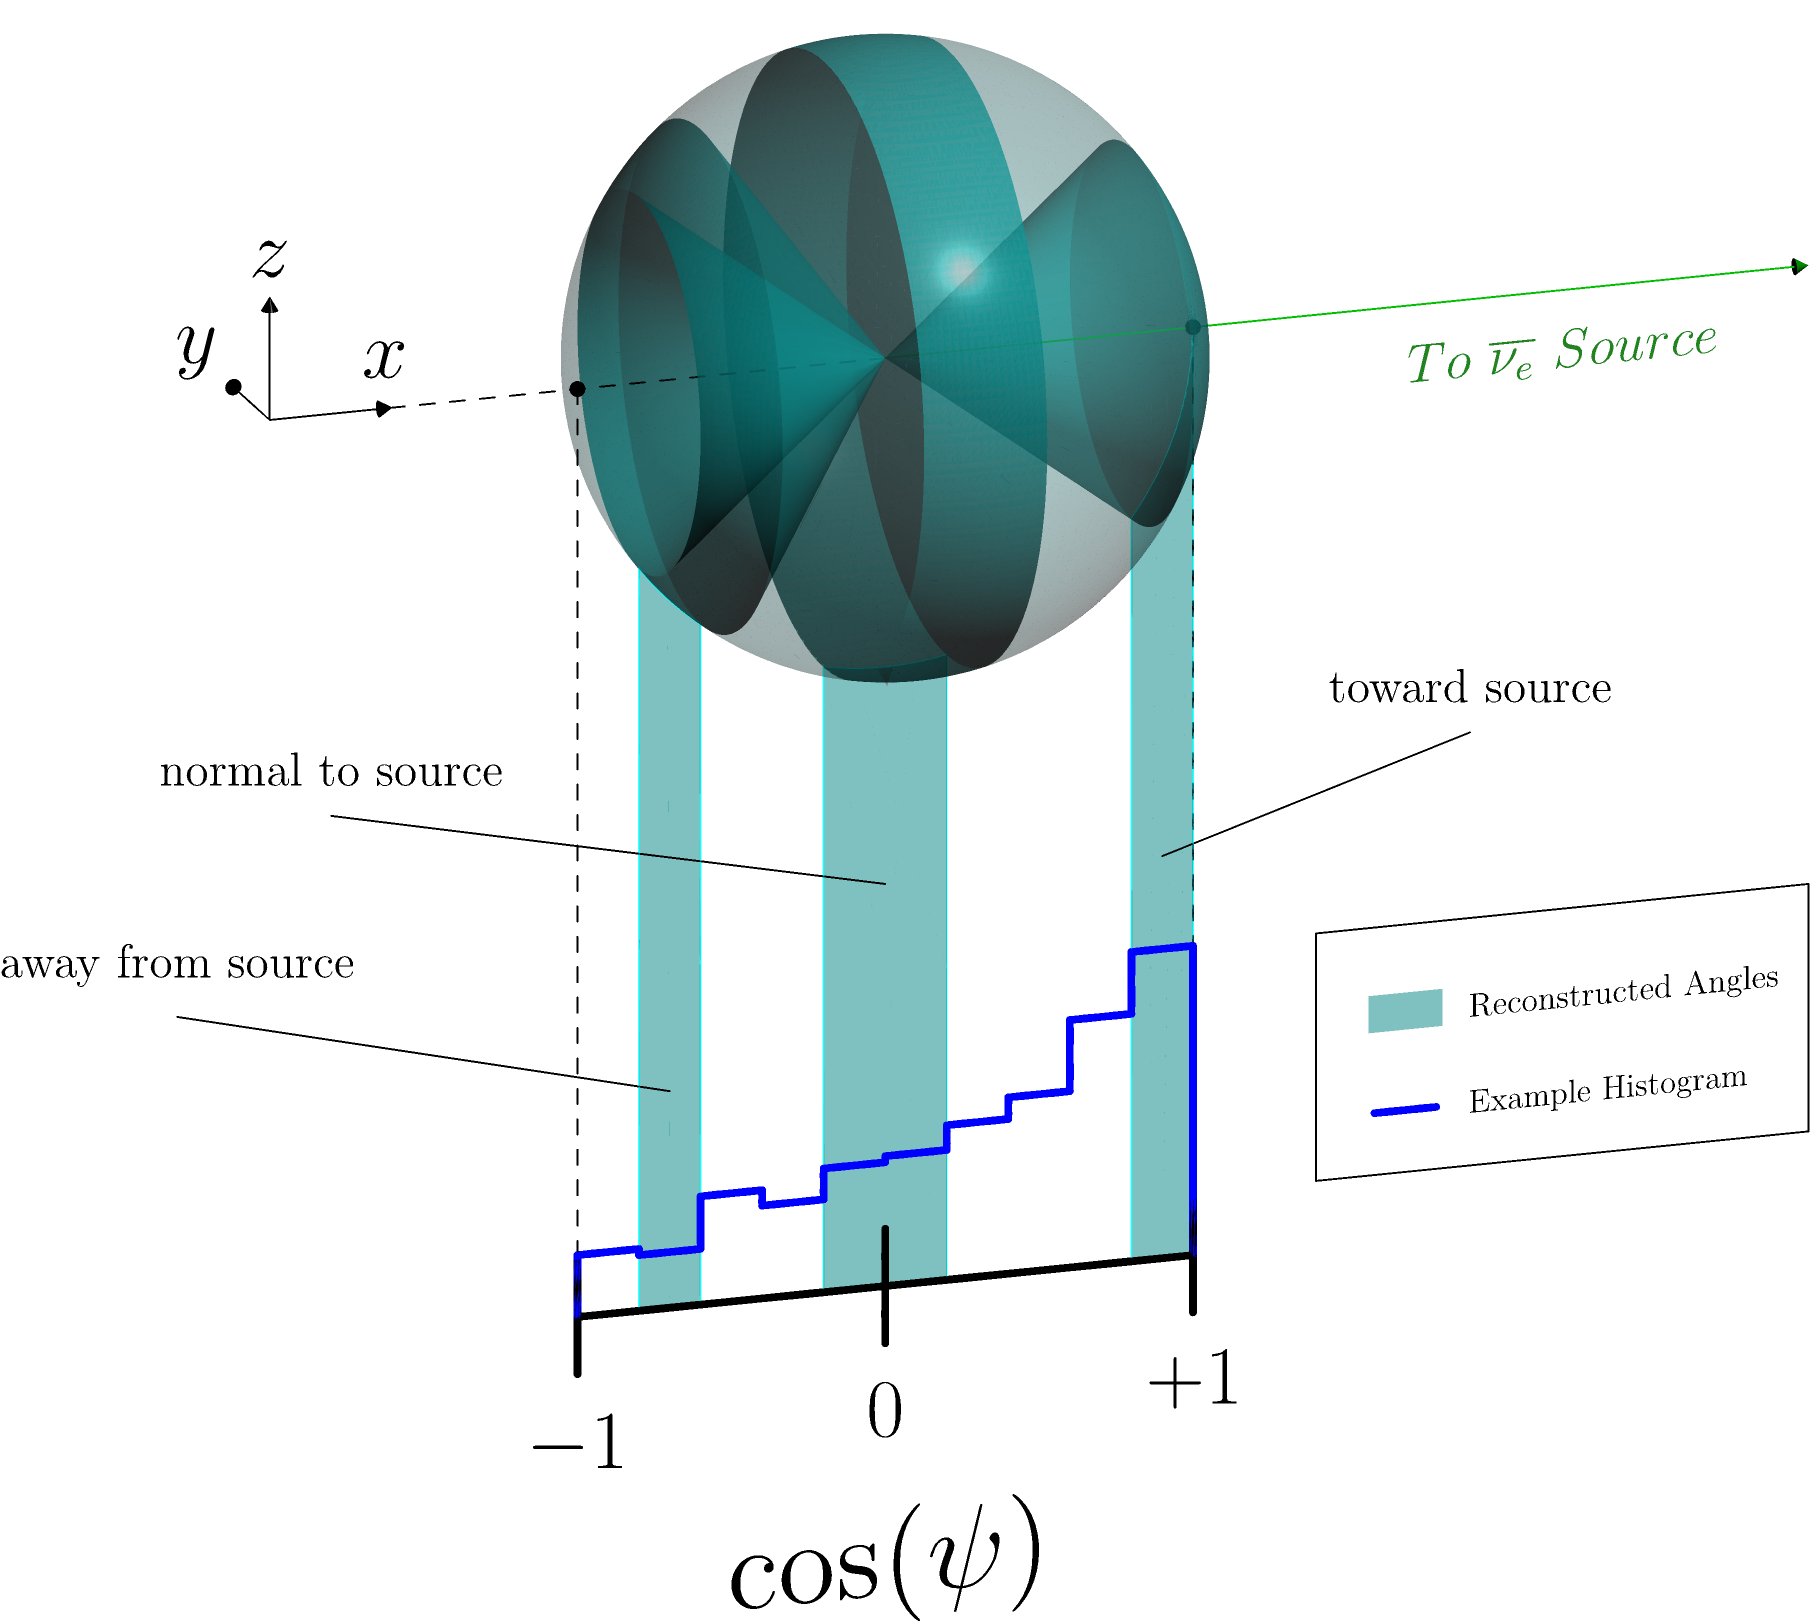
\includegraphics[width=1.0\linewidth]{figures/cospsi.png}
    \caption{\textbf{Physical Meaning of Cos$\bm{(\psi)}$ Distributions}}
    \label{fig:cospsi}
  \end{center}
\end{figure}

The angle $\psi$ \dash or more specifically, its cosine \dash is especially helpful for evaluating a detector's directional performance.
The quantity $\cos(\psi)$ for a given event or set of events gives a single value on the interval $\{-1,+1\}$ that reflects the degree of agreement between \rhat\ and \snu, as illustrated in Fig.~\ref{fig:cospsi}.
Values near $-1$ indicate a reconstructed direction pointing away from the true source direction; values near $0$, perpendicular to the true source direction; and values near $+1$, toward the true source direction.
For example, events in the leftmost shaded region in Fig.~\ref{fig:cospsi} (i.e., the second bin from the left in the example histogram) correspond to reconstructed angles falling within the solid angle between the two cones defined by $\cos(\psi) = -0.8$ and $\cos(\psi) = -0.6$, or $\psi \approx 143^o$ and $\psi \approx 127^o$.


% summary table
% \begin{sidewaystable}
% \begin{table}
\begin{table*}
  \begin{tabular}{ c | l | c | c | r | r | r | R | R | R | R | R }
    ~ & \textbf{Experiment} & \textbf{Material} & \textbf{Dopant} & \textbf{\%wt.} & \textbf{IBDs} & \textbf{Vol.~(L)} 
      & \bm{N_{trg}} & \bm{N_{1V}} & \bm{N~~} & \bm{ \overline{c\psi}~~ } & \bm{ [\Delta \varphi]_{1\sigma}~(^\circ) } \\ \hline %& \bm{ ~~\overline{c\psi}/N \times 10^{6}}\\ \hline
    %                & CHOOZ-type    & DC LOS  &             Gd & 0.1~ & 10~000 & 785~000\textcolor{white}{.00}  & 	 9198~			&\textbf{---}~		& 9198~			& 0.052~		&	6.4~~~\\ %& 5.65~\\
               & NuLat ($3^3$) & EJ-Base & $\nucl{6}{Li}$ & 1.5~ & 10~000 &      15.6\textcolor{white}{0}  & 	 5763^\emph{\dag}	& 829^\emph{\dag}	& 4934^\emph{\dag}	& 0.224^\emph{\dag}	&	1.4^\emph{\dag}~~\\ %& 45.40^\emph{\dag}\\
   \textit{3D} & NuLat ($5^3$) & EJ-Base & $\nucl{6}{Li}$ & 1.5~ & 10~000 &     422.\textcolor{white}{00}  & 	 4592~			& 661~			& 3931~			& 0.256~		&	1.1~~~\\ %& 65.20~\\
               & 3D Chkbd.     & EJ-Base & $\nucl{6}{Li}$ & 1.5~ & 10~000 &     107.\textcolor{white}{00}  & 	 4384~			& 178~			& 4206~			& 0.194~		&	0.68\,~\\ %& 46.10~\\
               & SANTA         & EJ-Base &              B & 0/5~ & 10~000 &      24.0\textcolor{white}{0}  & 	 2275~			& 0~			& 2275~			& 0.876~		&	0.032\\ \hline %& 385.00~\\ \hline
%	
               & SANDD-CM      & EJ-Base & $\nucl{6}{Li}$ & 1.5~ & 10~000 &       0.64                     & 	 250~			& 3~			& 247~			& 0.360~		&	2.0~~~\\ %& 1460.00~\\
   \textit{2D} & 2D Chkbd.     & EJ-Base & $\nucl{6}{Li}$ & 1.5~ & 10~000 &       5.12                     & 	 1864~			& 4~			& 1860~			& 0.297~		&	0.51\,~\\ %& 160.00~\\
               & PROSPECT      & EJ-Base & $\nucl{6}{Li}$ & 0.08 & 10~000 &   6~930\textcolor{white}{.00}  & 	 2257~			& 239~			& 2018~			& 0.335~		&	1.9~~~\\ %& 166.00~
 % magic happens here
                   & CHOOZ-type    & DC LOS  &             Gd & 0.1~ & 10~000 & 785~000\textcolor{white}{.00}  & 	 9198~			&\textbf{---}~		& 9198~			& 0.052~		&	6.4~~~\\ %& 5.65~\\
               & NuLat ($3^3$) & EJ-Base & $\nucl{6}{Li}$ & 1.5~ & 10~000 &      15.6\textcolor{white}{0}  & 	 5763^\emph{\dag}	& 829^\emph{\dag}	& 4934^\emph{\dag}	& 0.224^\emph{\dag}	&	1.4^\emph{\dag}~~\\ %& 45.40^\emph{\dag}\\
   \textit{3D} & NuLat ($5^3$) & EJ-Base & $\nucl{6}{Li}$ & 1.5~ & 10~000 &     422.\textcolor{white}{00}  & 	 4592~			& 661~			& 3931~			& 0.256~		&	1.1~~~\\ %& 65.20~\\
               & 3D Chkbd.     & EJ-Base & $\nucl{6}{Li}$ & 1.5~ & 10~000 &     107.\textcolor{white}{00}  & 	 4384~			& 178~			& 4206~			& 0.194~		&	0.68\,~\\ %& 46.10~\\
               & SANTA         & EJ-Base &              B & 0/5~ & 10~000 &      24.0\textcolor{white}{0}  & 	 2275~			& 0~			& 2275~			& 0.876~		&	0.032\\ \hline %& 385.00~\\ \hline
%	
               & SANDD-CM      & EJ-Base & $\nucl{6}{Li}$ & 1.5~ & 10~000 &       0.64                     & 	 250~			& 3~			& 247~			& 0.360~		&	2.0~~~\\ %& 1460.00~\\
   \textit{2D} & 2D Chkbd.     & EJ-Base & $\nucl{6}{Li}$ & 1.5~ & 10~000 &       5.12                     & 	 1864~			& 4~			& 1860~			& 0.297~		&	0.51\,~\\ %& 160.00~\\
               & PROSPECT      & EJ-Base & $\nucl{6}{Li}$ & 0.08 & 10~000 &   6~930\textcolor{white}{.00}  & 	 2257~			& 239~			& 2018~			& 0.335~		&	1.9~~~\\ %& 166.00~
 % magic happens here
  \end{tabular}
  \caption[\textbf{Summary Table of New Simulation Results}]{\textbf{Summary Table of New Simulation Results}\\
    ~\\
    % See~\ref{subsubsec:res_coldet}~for detailed descriptions of columns.\\
    See~\ref{list:res_coldet}~for detailed descriptions of columns.\\
    % \textsc{Note:} The 2D experiments are reconstructing the \textbf{azimuthal angle only}.\\
    Note that the 2D experiments are reconstructing the \textbf{azimuthal angle only}.}
    % ~\\
    % \underline{Column Details}\\
    % $\bm{\cdot}$ ``Material'': DC LOS is our simulated version of Double CHOOZ' liquid organic scintillator;\\
    %     \textcolor{white}{000} EJ-Base is our simulated version of EJ-254 (prior to doping).\\%, which is the base polymer (PVT) and the scintillator.\\%\footnotesize
    % $\bm{\cdot}$ ``Vol.'' is the detector's active target volume; SANTA's capture plane and the inert checkerboard cells are not included.\\
    % $\bm{\cdot}$ ``IBDs'' is the total number of IBDs simulated in each detector.\\
    % $\bm{\cdot}$ $N_{trg}$ is the total number of IBD-candidate events registered by the neutrino trigger.\\
    % $\bm{\cdot}$ $N_{1V}$ is the number of IBD-candidate events for which the prompt and delayed events occurred within a single volume;\\
    %     \textcolor{white}{000} these events were not used for directional reconstruction except in the single-volume (CHOOZ-type) detector.\\
    % $\bm{\cdot}$ $N = N_{trg} - N_{1V}$ is the resulting number of IBD-candidate events used for directional reconstruction.\\
    % $\bm{\cdot}$ $\overline{c\psi}\ \equiv\ \langle \cos(\psi) \rangle$, the mean of $\cos(\psi)$.\\
    % % $\bm{\cdot}$ $[\Delta \varphi]_{1\sigma}$ is the $1\sigma$ angular uncertainty on the reconstructed direction to the antineutrino source~\cite{Caden:2012aap};\\
    % $\bm{\cdot}$ $[\Delta \varphi]_{1\sigma}$ is the $1\sigma$ angular uncertainty on the reconstructed direction to the antineutrino source \dash see Appendix C~\{\ref{ch:deltaphi}\} for calculation;
 	% \textcolor{white}{000} it is the half-aperture of a cone in the 3D experiments and the half-angle of an arc in the 2D experiments.\\
    % % $\bm{\cdot}$ $[\Delta \varphi]_{1\sigma}$ is the half-aperture angle of a cone representing the $1\sigma$ uncertainty on the reconstructed source direction;\\
    % % 	\textcolor{white}{000} this is one way of defining the detector's angular resolution~\cite{Caden:2012aap}.\\
    % % $\bm{\cdot}$ $\overline{c\psi}/N \times 10^{6}$ is the mean $\cos(\psi)$ per event, scaled up by $10^{6}$ for readability\\
    %     % \textcolor{white}{0} \textbf{---} E.g., the actual value of $\langle \cos(\psi) \rangle / N$\ for the 3-D Checkerboard is  0.000461\\
    % ~\\
    % \emph{$^{\dag}$For the NuLat ($\mathit{3^3}$) experiment, IBDs were constrained to the central cube rather than distributed throughout the detector.}}%\normalsize
  \label{tab:ncomp_results}
% \end{sidewaystable}
% \end{table}
\end{table*}

% \underline{Column Details}\\
% \paragraph{Column Details for~\ref{tab:ncomp_results}}
% \subsubsection{\label{subsubsec:res_coldet}Column Details for~\ref{tab:ncomp_results}}
%\subsubsection*{\label{subsubsec:res_coldet}Column Details for Table~\ref{tab:ncomp_results}}
% \begin{itemize}[label=$\bm{\cdot}$]
%\paragraph{~\label{list:res_coldet}}

~\\
\textbf{Column Details for Tab.~\ref{tab:ncomp_results}:}\label{list:res_coldet}
\begin{itemize}[label=$\bm{\cdot}$]
    % \label{list:res_coldet}Column Details for~\ref{tab:ncomp_results}
  % \item ``Material'': DC LOS is our simulated version of Double CHOOZ' liquid organic scintillator;\\
  %     \textcolor{white}{000} EJ-Base is our simulated version of EJ-254 (prior to doping).\\%, which is the base polymer (PVT) and the scintillator.\\%\footnotesize
  \item ``Vol.'' is the detector's active target volume; SANTA's capture plane and the inert checkerboard cells are not included.
  \item ``IBDs'' is the total number of IBDs simulated in each detector.
  \item $N_{trg}$ is the total number of IBD-candidate events registered by the neutrino trigger.
  \item $N_{1V}$ is the number of IBD-candidate events for which the prompt and delayed events occurred within a single volume;
      \textcolor{white}{000} these events were not used for directional reconstruction except in the single-volume (CHOOZ-type) detector.
  \item $N = N_{trg} - N_{1V}$ is the resulting number of IBD-candidate events used for directional reconstruction.
  \item $\overline{c\psi}\ \equiv\ \langle \cos(\psi) \rangle$, the mean of $\cos(\psi)$.
  % \item $[\Delta \varphi]_{1\sigma}$ is the $1\sigma$ angular uncertainty on the reconstructed direction to the antineutrino source~\cite{Caden:2012aap};
  \item $[\Delta \varphi]_{1\sigma}$ is the $1\sigma$ angular uncertainty on the reconstructed direction to the antineutrino source \dash see Eq.~\ref{eq:deltaphi};
      \textcolor{white}{000} it is the half-aperture of a cone in the 3D experiments and the half-angle of an arc in the 2D experiments.
  % \item $[\Delta \varphi]_{1\sigma}$ is the half-aperture angle of a cone representing the $1\sigma$ uncertainty on the reconstructed source direction;
  % 	\textcolor{white}{000} this is one way of defining the detector's angular resolution~\cite{Caden:2012aap}.
  % \item $\overline{c\psi}/N \times 10^{6}$ is the mean $\cos(\psi)$ per event, scaled up by $10^{6}$ for readability
      % \textcolor{white}{0} \textbf{---} E.g., the actual value of $\langle \cos(\psi) \rangle / N$\ for the 3-D Checkerboard is  0.000461
\end{itemize}
~\\
\emph{$^{\dag}$For the NuLat ($\mathit{3^3}$) experiment, IBDs were constrained to the central cube rather than distributed throughout the detector.} %\normalsize



% end \section
